\cotefile{74}
\scanpage{19}

% L1–5
\[
\left\{\begin{aligned}
 &V\quad\text{groupe}\\
 &I\subset V\quad\text{partie de }V\\
 &V\xrightarrow{\varphi_\lambda}V_\lambda\quad(\lambda\in\Lambda)
 \quad\text{hom de groupes},\quad I_\lambda\subset V_\lambda\quad\text{partie de }V_\lambda\\
 &\deleted{\unsure{T|X}}\;Y\ \deleted{\unsure{\text{ens}}}\ \text{un }V\text{-ens.}
 \quad X_\lambda=\deleted{X}Y\mathbin{\wedge}_V(V_\lambda,\varphi_\lambda),\
 \text{d'où }\tau_\lambda:Y\mathbin{\unsure{-|\to}}X_\lambda\\
 &S=\deleted{\unsure{X_a|X}}\{a\}\amalg Y\amalg
 \overbrace{\coprod_{\lambda\in\Lambda}
 \underbrace{Y\times_V(V_\lambda,\varphi_\lambda)}_{X_\lambda}}^{X}
\end{aligned}\right.
\]

% L6
Structure de graphe sur $S$ :

% L7–10
\[
\left\{\begin{aligned}
 &\unsure{\{a\}|a|e}\ \text{est lié aux él. de } \deleted{\unsure{S_{\lambda,y}}}\,X\deleted{{}_{\unsure{\lambda|x}}}.\\
 &\deleted{\unsure{\text{les}}}\ y\in Y\ \text{est lié à }iy\quad(i\in I)\\
 &x\in X_\lambda\ \text{est lié à }ix\quad(i\in V_\lambda)\\
 &y\in Y\ \text{est lié à son image }\tau_\lambda(y)\in X_\lambda
\end{aligned}\right.
\]

% L11
et \unsure{celà|cela} épuise les arêtes.

% L12–14
À quelles conditions est-ce là un graphe trialitaire ? Je dis qu'il n'y a que les cas suivants

% L15
\[
 \text{a) }\ V\simeq\mathbb F_2^{\unsure{c_\nu|c_v|r}+1}\
 \deleted{\unsure{\nu\in\{2,3,4\}}}\ \text{où }c_\nu=
 \deleted{\unsure{\nu}}2^\nu\deleted{\unsure{+1}},\quad \nu\in\{0,1,2\}
\]

% L16
b) $I$ est une base de $V$

% L17
c)
% archive sheet number: 18
\scanpage{21}

% L1–3 upper left
\diagram{\begin{tikzcd}[ampersand replacement=\&,column sep=small,row sep=3ex]
 \& \underline{\unsure{\zeta|\xi}_1}\zeta_2\zeta_3
 \arrow[r,dash]\arrow[dl,dash]\arrow[dd,dash,dashed]\arrow[drr,dash,dashed]
 \& \underline{\zeta_4}\zeta_5\zeta_6
 \arrow[dr,dash]\arrow[dll,dash,dashed]\arrow[dd,dash,dashed] \& {}\\
 \underline{\zeta_{45}}\zeta_{56}\zeta_{64}\arrow[dr,dash]\arrow[drr,dash,dashed]
 \& \& \& \zeta_{23}\underline{\zeta_{31}}\zeta_{12}\arrow[dl,dash]\arrow[dll,dash,dashed]\\
 \& \underline{\zeta_{\deleted{\unsure{4}}1}^{\unsure{*|+}}}\zeta_2^*\zeta_3^*
 \arrow[r,dash]\& \underline{\zeta_4}\zeta_5^*\zeta_6^* \&
\end{tikzcd}}

% L1 top centre
\figure{\begin{tikzpicture}[scale=.5]\draw[->] (0,.6) .. controls (.45,.7) and (.8,.45) .. (1.1,0);\end{tikzpicture}}

% L1–2 upper right
\figure{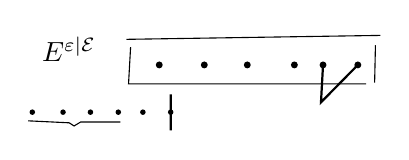
\begin{tikzpicture}[x=.52cm,y=.5cm]
\node at (-1,1.6) {$E^{\unsure{\varepsilon|\mathcal E}}$};
\draw (.4,1.85)--(6.6,1.95) (.5,1.65)--(.45,.72)--(6.25,.72) (6.48,1.7)--(6.46,.75);
\foreach \x in {1.2,2.3,3.35,4.5,5.2,6.05}{\fill (\x,1.2) circle (1.25pt);}
\foreach \x in {-1.9,-1.15,-.48,.2,.8,1.48}{\fill (\x,0) circle (1pt);}
\draw[thick] (5.2,1.2)--(5.15,.25)--(6.05,1.2) (1.48,.45)--(1.48,-.46);
\draw (-2,-.22)--(-1,-.27)--(-.88,-.35)--(-.72,-.25)--(.25,-.25);
\end{tikzpicture}}

% L3–4 upper right
(hexagone distingué ou triplet distingué

% L4 just below hexagon
$\unsure{\zeta_{14}|\zeta_1\,4}$

% L5–7 left
\deleted{2 ens à trois él. $E,E'$}

1 ens à trois él. $I$

% L7 left
\[
 E\times I\ \amalg\ E\times I'
\]

% L5–7 right
\[
\left\{\begin{aligned}
 &\text{ens à }\deleted{\unsure{3}}\!6\ \text{él. fibré \inserted{de degré 3} sur ens }\varepsilon\text{ à 2 él.}\\
 &\hspace{2em} E=\deleted{\unsure{E}}\coprod_{\alpha\in\varepsilon}E_\alpha\\
 &\text{ens à trois él. }I
\end{aligned}\right.
\]

% L8
\[
 I\times\varepsilon\quad\text{h\deleted{\unsure{a}}exagone}
\]

% L9 left
$\zeta_1\zeta_2\zeta_3$

% L9–12 centre
il y a 6 él. liés à aucun \uline{des $\zeta_i$}

il y a \unsure{3 él.|trois él.} \deleted{\unsure{sont}} liés à deux \unsure{$\zeta_\alpha$} \unsure{(pt E|$\alpha\in E$}

il y a 6 él. liés à exact 2 des $\zeta_i$

et 9 él. liés à exact un

% L9 right
\[
 E_\alpha\times I= E\mathbin{\unsure{\times|\alpha}}I\quad\text{fibré sur } I\mathbin{\times}\varepsilon
\]

% L12 lower centre
\[
 X=\prod_{\alpha\in\varepsilon}E_\alpha
\]

% foot, left to right
\figure{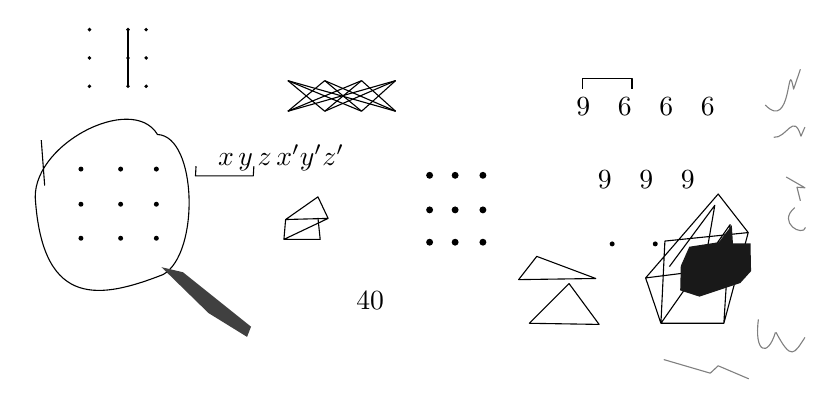
\begin{tikzpicture}[x=.72cm,y=.72cm,line join=round]
\foreach \x in {1.1,1.78,2.1}{\foreach \y in {4.4,4.9,5.4}{\fill (\x,\y) circle (.7pt);}}
\draw (1.78,4.4)--(1.78,5.4);
\draw (.15,2.35) .. controls (.02,3.35) and (1.85,4.3) .. (2.3,3.55) .. controls (3,3.52) and (3.05,1.45) .. (2.4,1.08) .. controls (1.3,.65) and (.3,.48) .. (.15,2.35);
\draw (.25,3.45)--(.31,2.65);
\foreach \x in {.95,1.65,2.28}{\foreach \y in {1.72,2.32,2.94}{\fill (\x,\y) circle (.9pt);}}
\fill[black!75] (2.37,1.21)--(2.75,1.12)--(3.95,.16)--(3.88,-.02)--(3.2,.4)--cycle;

\node at (4.48,3.14) {$x\,y\,z\,x'y'z'$};
\draw (2.98,2.99)--(2.97,2.82)--(3.99,2.82)--(4,2.99);
\foreach \x/\t in {4.6/5.25,4.6/5.9,4.6/6.5,5.25/4.6,5.25/5.9,5.25/6.5,5.9/4.6,5.9/5.25,5.9/6.5,6.5/4.6,6.5/5.25,6.5/5.9}{\draw[thin] (\x,4.5)--(\t,3.96);}
\draw (4.53,1.7)--(4.56,2.05)--(5.13,2.45)--(5.31,2.07)--(4.56,2.05) (5.31,2.07)--(4.53,1.7)--(5.17,1.7)--(5.13,2.08);
\foreach \x in {7.1,7.55,8.04}{\foreach \y in {1.65,2.22,2.83}{\fill (\x,\y) circle (1.25pt);}}
\node at (6.05,.62) {$40$};
\node at (10.91,4.04) {$9\quad 6\quad 6\quad 6$};
\draw (9.8,4.36)--(9.8,4.54)--(10.67,4.54)--(10.67,4.36);
\node at (10.92,2.76) {$9\quad 9\quad 9$};
\fill (10.32,1.62) circle (.9pt); \fill (11.08,1.62) circle (.9pt);
\draw (8.67,.99)--(8.99,1.4)--(10.03,1.01)--cycle (8.86,.22)--(9.56,.92)--(10.09,.2)--cycle;
\draw (10.91,1.02)--(12.19,2.5)--(12.72,1.82)--(12.29,.22)--(11.18,.22)--cycle
 (11.18,.22)--(11.25,1.67)--(12.72,1.82) (10.91,1.02)--(12.5,1.22)
 (11.18,.22)--(12.4,1.96)--(12.29,.22) (11.33,1.22)--(12.13,2.3)--(11.92,1.08);
\fill[black!90] (11.53,1.23)--(11.68,1.57)--(12.2,1.65)--(12.43,1.95)--(12.45,1.63)--(12.76,1.63)--(12.77,1.14)--(12.58,.93)--(11.86,.69)--(11.52,.8)--cycle;
\draw[gray,thin] (13.02,4.07) .. controls (13.5,3.58) and (13.4,4.98)..(13.52,4.35)--(13.64,4.7)
 (13.17,3.5) .. controls (13.4,3.48) and (13.52,3.95)..(13.65,3.52)--(13.72,3.68)
 (13.39,2.8)--(13.72,2.61)--(13.58,2.62)--(13.64,2.38)
 (13.54,2.26) .. controls (13.22,1.99) and (13.69,1.74)..(13.73,1.91)
 (12.9,.29) .. controls (12.82,-.29) and (13.06,-.4)..(13.2,.06)
 (13.21,.06) .. controls (13.48,-.45) and (13.53,-.32)..(13.72,-.03)
 (11.23,-.42)--(12.05,-.66)--(12.19,-.53)--(12.73,-.76);
\end{tikzpicture}}
% crop-candidate: scan 21
% archive sheet number: 20
\scanpage{22}

\handwritten{%
% L1–3 upper left
\[
 \begin{aligned}
 B\quad\underline{B'\amalg B''}\qquad&
 \unsure{\zeta|\xi}_{14}\ \zeta_{15}\ \zeta_{16}\\
 &\zeta_{\unsure{24|23}}\ \zeta_{25}\ \zeta_{\unsure{26|22}}\\
 &\zeta_{24}\ \zeta_{\unsure{25|35}}\ \zeta_{26}
 \end{aligned}
\]

% L2–3 upper left
\figure{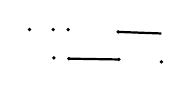
\begin{tikzpicture}[scale=.5]
\foreach \p in {(0,1),(.6,1),(.98,1),(2.25,.94),(.62,.28),(1,.26),(2.27,.24),(3.35,.18)}{\fill \p circle (1.35pt);}
\draw[thick] (1,.26)--(2.27,.24) (2.25,.94)--(3.35,.9);
\end{tikzpicture}}

% L1–5 upper centre
\[
 \begin{array}{r}36\\36\\\hline216\\108\phantom{0}\\\hline1296\\1440\end{array}
 \qquad 
\begin{tikzpicture}[scale=.35]\foreach \y in {0,.45,.9}{\draw (0,\y)--(.85,\y-.5);}\end{tikzpicture}
\]

% L4–5 left
\figure{\begin{tikzpicture}[scale=.45]\foreach \x in {0,.7}{\foreach \y in {0,.55,1.1}{\fill (\x,\y) circle (1.25pt);}}\draw (-.3,.78)--(-.2,-.2);\end{tikzpicture}}

% L5
$\ldots$ trièdres $\longleftrightarrow$ hexagones

% L6–7
\[
 \begin{aligned}
 6^4&=36\mathbin{\unsure{\times|<}}36=2^4\,3^4\\
 720&=\underline{2^{\unsure{4|3}}\cdot3^2}\cdot5.\qquad 9/5
 \end{aligned}
 \qquad
 \left\{\begin{array}{l}40\\\deleted{45}\,36\\45\end{array}\right.
\]

% L8 between horizontal rules
\unsure{Problème|Partons|Partition} \unsure{orbitier|plutôt|ordonnée} d'un \deleted{\unsure{tri}}

% L9
\[
 \zeta_{12}\ \zeta_{23}\ \zeta_{31}\ \big|\ \zeta_{45}\
 \overset{\leftrightarrow}{\check{\zeta}_{56}}\ \zeta_{64}
\]

% L10–14 middle left
\figure{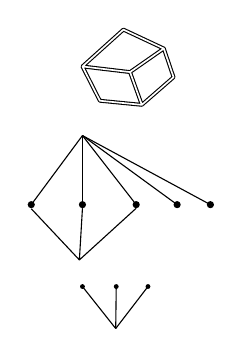
\begin{tikzpicture}[scale=.65,line join=round]
\draw[double] (0,2.7)--(.8,3.42)--(1.59,3.05)--(1.78,2.49)--(1.16,1.95)--(.34,2.03)--cycle (0,2.7)--(.93,2.59)--(1.59,3.05) (.93,2.59)--(1.16,1.95);
\foreach \x in {-1,0,1.05,1.85,2.5}{\draw (0,1.35)--(\x,0);\fill (\x,0) circle (2pt);}
\draw (-1,-.08)--(-.06,-1.08)--(1.05,-.07) (-.06,-1.08)--(0,-.07);
\foreach \x in {0,.66,1.28}{\draw (.65,-2.42)--(\x,-1.6);\fill (\x,-1.6) circle (1.35pt);}
\end{tikzpicture}}

% L10–13 middle right
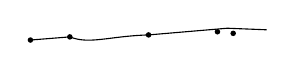
\begin{tikzpicture}[x=.5cm,y=.5cm]\draw (0,0)--(1,.08)..controls (1.5,-.12) and (2,.1)..(3,.13)--(5,.3)--(6,.26);\foreach \x/\y in {0/0,1/.08,3/.13,4.75/.21,5.15/.17}{\fill (\x,\y) circle (1pt);}\end{tikzpicture}

\unsure{se répartissent} en \unsure{liés au}

$\deleted{\unsure{\zeta}}\zeta_{ij}\qquad \deleted{\unsure{\zeta}}\zeta_{ij}\quad i,j\in\{1,\ldots,6\}$

\unsure{en} \unsure{iBs|i et j} $\longrightarrow$ non liés

% L14 middle right
\[
 \zeta_{12}\ \zeta_{13}\ -\ \zeta_{16}
\]

}
% printed form, rotated 180 degrees, left column
% printed form
N\textsuperscript{o}

UNIVERSITÉ DES SCIENCES\\
ET TECHNIQUES\\
DU LANGUEDOC

(1) -- Le candidat doit indiquer la nature de l'examen auquel il se présente.

(2) -- Le candidat inscrit ses nom, prénom, lieu et date de naissance en tête de la copie et signe lisiblement son nom à la fin de la composition.

% printed form, rotated 180 degrees, main column
% printed form
ACADEMIE DE MONTPELLIER

\textit{Examen de} \textsuperscript{(1)} \dotfill\\
\mbox{}\dotfill

\textit{Nom et Prénoms du Candidat} \textsuperscript{(2)} \dotfill

\textit{né à} \dotfill\quad \textit{département de} \dotfill

\textit{le} \dotfill\quad 19

\textit{Montpellier, le} \dotfill\quad 19

COMPOSITION EN \dotfill
% archive sheet number: 21
\scanpage{23}

% top L1–8
\diagram{\begin{tikzcd}[ampersand replacement=\&,column sep=.2em,row sep=.55em,cells={nodes={inner sep=1pt}},font=\scriptsize]
 \& \underset{\overbrace{\hspace{2.4em}}}{\{1,2,3\}=I_3} \&  \&  \&  \&  \&  \&  \& \underset{\overbrace{\hspace{2.4em}}}{\{4,5,6\}=} \&  \& \boxed{\unsure{\mathcal T|\tau}_3}\arrow[from=1-11,to=2-10,dash,end anchor=north east] \\
\unsure{\zeta|\xi}_1 \& \zeta_{2} \& \zeta_{3}\arrow[from=2-3,to=2-8,dash]\arrow[from=2-3,to=4-8,dash,densely dashed] \&  \&  \&  \&  \& \zeta_{4} \& \zeta_{5} \& \zeta_{6} \&  \\
\zeta_{1}^{*} \& \zeta_{2}^{*} \& \zeta_{3}^{*}\arrow[from=3-3,to=3-8,dash]\arrow[from=3-3,to=4-8,dash,densely dashed] \&  \&  \&  \&  \& \zeta_{4}^{*} \& \zeta_{5}^{*} \& \zeta_{6}^{*} \& \left.\vphantom{\begin{matrix}X\\X\\X\end{matrix}}\right\}I_1=\{\unsure{?|2},*,!\} \\
\zeta_{23}\arrow[from=4-1,to=6-4,dash]\arrow[from=4-1,to=8-4,dash] \& \zeta_{31}\arrow[from=4-2,to=6-4,dash]\arrow[from=4-2,to=7-4,dash] \& \zeta_{12}\arrow[from=4-3,to=2-8,dash]\arrow[from=4-3,to=3-8,dash]\arrow[from=4-3,to=7-4,dash]\arrow[from=4-3,to=8-4,dash] \&  \&  \&  \&  \& \zeta_{56}\arrow[from=4-8,to=6-4,dash]\arrow[from=4-8,to=6-6,dash] \& \zeta_{64}\arrow[from=4-9,to=6-4,dash,densely dashed]\arrow[from=4-9,to=6-5,dash,densely dashed] \& \zeta_{45}\arrow[from=4-10,to=6-5,dash]\arrow[from=4-10,to=6-6,dash] \&  \\
 \&  \&  \&  \&  \&  \&  \&  \&  \&  \&  \\
 \&  \&  \& \zeta_{14} \& \zeta_{15} \& \zeta_{16} \&  \&  \&  \&  \&  \\
 \&  \&  \& \zeta_{24} \& \zeta_{25} \& \zeta_{26} \&  \&  \& \left.\vphantom{\begin{matrix}X\\X\\X\end{matrix}}\right\}\{1,2,3\}=I_3 \&  \&  \\
 \&  \&  \& \zeta_{34} \& \zeta_{35} \& \zeta_{36}\arrow[from=8-6,to=9-8,dash] \&  \&  \&  \&  \&  \\
 \&  \&  \&  \& \underbrace{\hspace{3em}}_{\{4,5,6\}} \&  \&  \& \text{\textcircled{\(\unsure{\mathcal T|\tau}_1\)}} \&  \&  \& 
\end{tikzcd}}

% middle right
\diagram{\begin{tikzcd}[ampersand replacement=\&,execute at end picture={\begin{scope}[x=.85cm,y=.85cm]\coordinate (v000) at (0.3,1.6);
\coordinate (v001) at (1.02,1.6);
\coordinate (v002) at (1.74,1.6);
\coordinate (v010) at (-0.06,0.9500000000000001);
\coordinate (v011) at (0.66,0.9500000000000001);
\coordinate (v012) at (1.38,0.9500000000000001);
\coordinate (v020) at (-0.42,0.30000000000000004);
\coordinate (v021) at (0.30000000000000004,0.30000000000000004);
\coordinate (v022) at (1.02,0.30000000000000004);
\coordinate (v100) at (4.8,1.44);
\coordinate (v101) at (5.52,1.44);
\coordinate (v102) at (6.24,1.44);
\coordinate (v110) at (5.2299999999999995,0.7999999999999999);
\coordinate (v111) at (5.949999999999999,0.7999999999999999);
\coordinate (v112) at (6.67,0.7999999999999999);
\coordinate (v120) at (5.66,0.15999999999999992);
\coordinate (v121) at (6.38,0.15999999999999992);
\coordinate (v122) at (7.1000000000000005,0.15999999999999992);
\coordinate (v200) at (3.3,4.65);
\coordinate (v201) at (3.8499999999999996,5.220000000000001);
\coordinate (v202) at (4.4,5.79);
\coordinate (v210) at (3.61,4.03);
\coordinate (v211) at (4.159999999999999,4.6000000000000005);
\coordinate (v212) at (4.71,5.17);
\coordinate (v220) at (3.92,3.41);
\coordinate (v221) at (4.47,3.9800000000000004);
\coordinate (v222) at (5.0200000000000005,4.55);
\draw (v000)--(v001)--(v002);
\draw (v000)--(v010)--(v020);
\draw (v010)--(v011)--(v012);
\draw (v001)--(v011)--(v021);
\draw (v020)--(v021)--(v022);
\draw (v002)--(v012)--(v022);
\draw (v100)--(v101)--(v102);
\draw (v100)--(v110)--(v120);
\draw (v110)--(v111)--(v112);
\draw (v101)--(v111)--(v121);
\draw (v120)--(v121)--(v122);
\draw (v102)--(v112)--(v122);
\draw (v200)--(v201)--(v202);
\draw (v200)--(v210)--(v220);
\draw (v210)--(v211)--(v212);
\draw (v201)--(v211)--(v221);
\draw (v220)--(v221)--(v222);
\draw (v202)--(v212)--(v222);
\draw (v001)--(v211)--(v101);
\draw (v011)--(v111);
\draw (v011)--(v112);
\fill (v000) circle (1.15pt);\node[above,inner sep=1.2pt] at (v000) {$\zeta_{1}$};
\fill (v001) circle (1.15pt);\node[above,inner sep=1.2pt] at (v001) {$\zeta_{2}$};
\fill (v002) circle (1.15pt);\node[above,inner sep=1.2pt] at (v002) {$\zeta_{3}$};
\fill (v010) circle (1.15pt);\node[left,inner sep=1.2pt] at (v010) {$\zeta_{1}^*$};
\fill (v011) circle (1.15pt);\node[below right,inner sep=1.2pt] at (v011) {$\zeta_{2}^*$};
\fill (v012) circle (1.15pt);\node[right,inner sep=1.2pt] at (v012) {$\zeta_{3}^*$};
\fill (v020) circle (1.15pt);\node[below,inner sep=1.2pt] at (v020) {$\zeta_{23}$};
\fill (v021) circle (1.15pt);\node[below,inner sep=1.2pt] at (v021) {$\zeta_{31}$};
\fill (v022) circle (1.15pt);\node[below,inner sep=1.2pt] at (v022) {$\zeta_{12}$};
\fill (v100) circle (1.15pt);\node[above,inner sep=1.2pt] at (v100) {$\zeta_{4}$};
\fill (v101) circle (1.15pt);\node[above,inner sep=1.2pt] at (v101) {$\zeta_{5}$};
\fill (v102) circle (1.15pt);\node[above,inner sep=1.2pt] at (v102) {$\zeta_{6}$};
\fill (v110) circle (1.15pt);\node[left,inner sep=1.2pt] at (v110) {$\zeta_{4}^*$};
\fill (v111) circle (1.15pt);\node[below right,inner sep=1.2pt] at (v111) {$\zeta_{5}^*$};
\fill (v112) circle (1.15pt);\node[right,inner sep=1.2pt] at (v112) {$\zeta_{6}^*$};
\fill (v120) circle (1.15pt);\node[below,inner sep=1.2pt] at (v120) {$\zeta_{56}$};
\fill (v121) circle (1.15pt);\node[below,inner sep=1.2pt] at (v121) {$\zeta_{64}$};
\fill (v122) circle (1.15pt);\node[below,inner sep=1.2pt] at (v122) {$\zeta_{45}$};
\fill (v200) circle (1.15pt);\node[left,inner sep=1.2pt] at (v200) {$\zeta_{14}$};
\fill (v201) circle (1.15pt);\node[above left,inner sep=1.2pt] at (v201) {$\zeta_{15}$};
\fill (v202) circle (1.15pt);\node[above,inner sep=1.2pt] at (v202) {$\zeta_{16}$};
\fill (v210) circle (1.15pt);\node[left,inner sep=1.2pt] at (v210) {$\zeta_{24}$};
\fill (v211) circle (1.15pt);\node[below right,inner sep=1.2pt] at (v211) {$\zeta_{25}$};
\fill (v212) circle (1.15pt);\node[right,inner sep=1.2pt] at (v212) {$\zeta_{26}$};
\fill (v220) circle (1.15pt);\node[below,inner sep=1.2pt] at (v220) {$\zeta_{34}$};
\fill (v221) circle (1.15pt);\node[below right,inner sep=1.2pt] at (v221) {$\zeta_{35}$};
\fill (v222) circle (1.15pt);\node[right,inner sep=1.2pt] at (v222) {$\zeta_{36}$};
\end{scope}}] {} \end{tikzcd}}

% middle right below miniature
$I$

% lower L1–6
\diagram{\begin{tikzcd}[ampersand replacement=\&,column sep=.2em,row sep=.55em,cells={nodes={inner sep=1pt}},font=\scriptsize]
 \&  \&  \&  \& \zeta_{14} \& \zeta_{15} \& \zeta_{16} \&  \&  \&  \&  \\
 \&  \&  \&  \& \zeta_{24} \& \zeta_{25} \& \zeta_{26} \&  \&  \&  \&  \\
 \&  \&  \&  \& \zeta_{34} \& \zeta_{35} \& \zeta_{36} \&  \&  \&  \&  \\
 \&  \&  \&  \&  \&  \&  \&  \&  \&  \&  \\
\zeta_{1}\arrow[from=5-1,to=2-5,dash]\arrow[from=5-1,to=3-5,dash] \& \zeta_{2}\arrow[from=5-2,to=1-5,dash,densely dashed]\arrow[from=5-2,to=3-5,dash,densely dashed] \& \zeta_{3}\arrow[from=5-3,to=5-9,dash]\arrow[from=5-3,to=7-9,dash,densely dashed]\arrow[from=5-3,to=1-5,dash]\arrow[from=5-3,to=2-5,dash] \&  \&  \&  \&  \&  \& \zeta_{4} \& \zeta_{5} \& \zeta_{6} \\
\zeta_{1}^{*} \& \zeta_{2}^{*} \& \zeta_{3}^{*}\arrow[from=6-3,to=6-9,dash]\arrow[from=6-3,to=7-9,dash,densely dashed] \&  \&  \&  \&  \&  \& \zeta_{4}^{*} \& \zeta_{5}^{*} \& \zeta_{6}^{*} \\
\zeta_{23} \& \zeta_{31} \& \zeta_{12}\arrow[from=7-3,to=5-9,dash]\arrow[from=7-3,to=6-9,dash] \&  \&  \&  \&  \&  \& \zeta_{56} \& \zeta_{64} \& \zeta_{45}
\end{tikzcd}}
% archive sheet number: 22
\scanpage{24}

% L1–2 upper left
$q\deleted{\unsure{,p}},q',a$ fixes

$p,p'$ échangés

% L1 upper centre
$p\,q\,p'\,q'\quad\deleted{\unsure{p}}$

% upper right
\diagram{\begin{tikzcd}[ampersand replacement=\&,execute at end picture={\begin{scope}[x=.72cm,y=.72cm]\coordinate (p) at (0,1);
\coordinate (q) at (1.5,1);
\coordinate (pp) at (1.5,0);
\coordinate (qp) at (0,0);
\draw[dashed] (p)--(q)--(pp)--(qp)--(p);
\fill (p) circle (1.15pt);\node[left,inner sep=1.2pt] at (p) {$p$};
\fill (q) circle (1.15pt);\node[right,inner sep=1.2pt] at (q) {$q$};
\fill (pp) circle (1.15pt);\node[right,inner sep=1.2pt] at (pp) {$p'$};
\fill (qp) circle (1.15pt);\node[left,inner sep=1.2pt] at (qp) {$q'$};
\end{scope}}] {} \end{tikzcd}}

% upper left main figure
\diagram{\begin{tikzcd}[ampersand replacement=\&,execute at end picture={\begin{scope}[x=.72cm,y=.72cm]\coordinate (q) at (2,7);
\coordinate (Q) at (3.3,5.9);
\coordinate (s) at (0,3.25);
\coordinate (R) at (2.55,3.35);
\coordinate (r) at (1.1,2.1);
\coordinate (S) at (3.85,2.25);
\coordinate (a) at (2,2.73);
\coordinate (p) at (.15,0);
\coordinate (P) at (2.45,.04);
\draw (q)--(Q)--(S)--(P)--(p)--(s)--(q);
\draw[->] (s)--(R)--(S)--(r)--(s);
\draw (p)--(r)--(Q);
\draw (p)--(a)--(Q);
\draw (P)--(R);
\draw[very thick] (q)--(a);
\draw (a)--(P);
\fill (q) circle (1.15pt);\node[above right,inner sep=1.2pt] at (q) {$q$};
\fill (Q) circle (1.15pt);\node[above right,inner sep=1.2pt] at (Q) {$q'$};
\fill (s) circle (1.15pt);\node[left,inner sep=1.2pt] at (s) {$s$};
\fill (R) circle (1.15pt);\node[above right,inner sep=1.2pt] at (R) {$r'$};
\fill (r) circle (1.15pt);\node[left,inner sep=1.2pt] at (r) {$r$};
\fill (S) circle (1.15pt);\node[right,inner sep=1.2pt] at (S) {$s'$};
\fill (a) circle (1.15pt);\node[right,inner sep=1.2pt] at (a) {$a$};
\fill (p) circle (1.15pt);\node[below,inner sep=1.2pt] at (p) {$p$};
\fill (P) circle (1.15pt);\node[below,inner sep=1.2pt] at (P) {$p'$};
\draw (q)--++(-.36,.46) (q)--++(.23,-2.25) (P)--++(-.58,.05) (p)--++(.89,1.9);
\draw[->] (P)--(3.03,1.05);\end{scope}}] {} \end{tikzcd}}

% L3–9 upper right
\deleted{\unsure{$r$ et $s$}}

$x$ et $y$ (distincts des 9 \unsure{pts|Vts} marqués) sont liés \unsure{exactemt|exclusivt|exactement}, parmi ces \unsure{pts|Vts}, l'un à $(r,a,r')$ l'autre à $(s\ a\ s')$.

Montrer que \inserted{si} $x,y$ sont \inserted{liés, ils \unsure{appart}} \deleted{\unsure{en totel. ils|liés, i.e.}} à un $=$ orbite

% L10–12 mid-page
$\underset{x\ne y}{x,y\in T'}$ pour qu'ils soient liés, il f et s. qu'ils aient des orbites distinctes, et \unsure{correspondent|convergentes} à des ombres distinctes sur $T$

% middle left
\diagram{\begin{tikzcd}[ampersand replacement=\&,execute at end picture={\begin{scope}[x=.72cm,y=.72cm]\coordinate (c) at (0,0);
\coordinate (b) at (2.6,0);
\coordinate (a) at (1.72,.85);
\coordinate (k) at (.15,1.28);
\coordinate (k1) at (.89,1.83);
\coordinate (s) at (1.98,1.96);
\coordinate (S) at (2.73,2.55);
\coordinate (t) at (2.86,1.35);
\coordinate (T) at (3.81,1.83);
\draw (c)--(b)--(t)--(k)--(c);
\draw (c)--(k1)--(S)--(T)--(b);
\draw (c)--(a)--(b);
\draw (a)--(s)--(S);
\draw (s)--(t)--(T);
\draw (k)--(k1)--(T);
\draw (k)--(s);
\fill (c) circle (1.15pt);\node[below left,inner sep=1.2pt] at (c) {$c$};
\fill (b) circle (1.15pt);\node[below right,inner sep=1.2pt] at (b) {$b$};
\fill (a) circle (1.15pt);\node[right,inner sep=1.2pt] at (a) {$a$};
\fill (k) circle (1.15pt);\node[left,inner sep=1.2pt] at (k) {$\unsure{\mu|k|a}$};
\fill (k1) circle (1.15pt);\node[above left,inner sep=1.2pt] at (k1) {$\unsure{k'|a'}$};
\fill (s) circle (1.15pt);\node[above left,inner sep=1.2pt] at (s) {$s$};
\fill (S) circle (1.15pt);\node[above right,inner sep=1.2pt] at (S) {$s'$};
\fill (t) circle (1.15pt);\node[above,inner sep=1.2pt] at (t) {$t$};
\fill (T) circle (1.15pt);\node[above right,inner sep=1.2pt] at (T) {$t'$};
\draw (a) circle (3pt) (t) circle (4pt);\end{scope}}] {} \end{tikzcd}}

% middle centre
\diagram{\begin{tikzcd}[ampersand replacement=\&,execute at end picture={\begin{scope}[x=.72cm,y=.72cm]\coordinate (a) at (0,1.1);
\coordinate (b) at (.9,1.07);
\coordinate (c) at (1.7,1.07);
\coordinate (t) at (3,2.1);
\coordinate (u) at (2.8,0);
\draw (a)--(t)--(u)--(a);
\draw (b)--(t);
\draw (c)--(t);
\draw (b)--(u);
\draw (c)--(u);
\fill (a) circle (1.15pt);
\fill (b) circle (1.15pt);
\fill (c) circle (1.15pt);
\fill (t) circle (1.15pt);
\fill (u) circle (1.15pt);
\end{scope}}] {} \end{tikzcd}}

% middle right
\figure{\begin{tikzpicture}[scale=.52]\foreach \x in {0,1,2}{\foreach \y in {0,1,2}{\fill (\x,\y) circle (1.5pt);}}\draw (3.9,3.6) .. controls (3.7,4.2) and (4.6,3.7) .. (4.03,3.58) .. controls (3.5,3.3) and (4.15,3.18) .. (4.15,3.44) .. controls (4.43,3.85) and (4.66,3.32) .. (5.25,3.5)--(5.42,3.32);\end{tikzpicture}}

% lower left
\diagram{\begin{tikzcd}[ampersand replacement=\&,execute at end picture={\begin{scope}[x=.72cm,y=.72cm]\coordinate (S) at (1.65,5.9);
\coordinate (a) at (1.05,4.12);
\coordinate (B) at (0,3.25);
\coordinate (C) at (2.19,3.39);
\coordinate (c) at (.43,2.05);
\coordinate (b) at (2.45,2.29);
\coordinate (A) at (1.08,1.59);
\coordinate (s) at (1.12,0);
\coordinate (al) at (1.16,3.2);
\coordinate (be) at (1.38,2.89);
\coordinate (ga) at (1.38,2.65);
\draw (B)--(S)--(C)--(b)--(s)--(c)--(B);
\draw (B)--(a)--(C);
\draw (B)--(be);
\draw (b)--(ga);
\draw (c)--(A)--(b);
\draw (a)--(al)--(A);
\draw (S)--(ga);
\fill (S) circle (1.15pt);\node[above,inner sep=1.2pt] at (S) {$s'$};
\fill (a) circle (1.15pt);\node[above,inner sep=1.2pt] at (a) {$a$};
\fill (B) circle (1.15pt);\node[left,inner sep=1.2pt] at (B) {$b'$};
\fill (C) circle (1.15pt);\node[right,inner sep=1.2pt] at (C) {$c'$};
\fill (c) circle (1.15pt);\node[left,inner sep=1.2pt] at (c) {$c$};
\fill (b) circle (1.15pt);\node[right,inner sep=1.2pt] at (b) {$b$};
\fill (A) circle (1.15pt);\node[below,inner sep=1.2pt] at (A) {$a'$};
\fill (s) circle (1.15pt);\node[below,inner sep=1.2pt] at (s) {$s$};
\fill (al) circle (1.15pt);\node[right,inner sep=1.2pt] at (al) {$\alpha$};
\fill (be) circle (1.15pt);\node[right,inner sep=1.2pt] at (be) {$\beta$};
\fill (ga) circle (1.15pt);\node[below right,inner sep=1.2pt] at (ga) {$\gamma$};
\draw (S) .. controls (2.04,5.42) and (2.17,4.22)..(C); \draw (.9,3.4)--(.95,3.91) (.77,2.72)--(.78,3.04) (.76,1.61)--(s) (c)--(.92,2.36);\end{scope}}] {} \end{tikzcd}}

% lower right
\diagram{\begin{tikzcd}[ampersand replacement=\&,execute at end picture={\begin{scope}[x=.72cm,y=.72cm]\coordinate (s) at (1.39,5.55);
\coordinate (a) at (0,3.13);
\coordinate (A) at (2.78,2.89);
\coordinate (B) at (1,4);
\coordinate (c) at (2.19,3.83);
\coordinate (C) at (.59,1.96);
\coordinate (b) at (2.06,1.85);
\coordinate (S) at (1.07,0);
\draw (s)--(a)--(C)--(S)--(A)--(c)--(s);
\draw (a)--(B)--(c);
\draw (C)--(b)--(A);
\draw (B)--(C);
\draw (s)--(b);
\draw[very thick] (s)--(1.18,2.16) (1.16,1.65)--(S);
\fill (s) circle (1.15pt);\node[above,inner sep=1.2pt] at (s) {$s$};
\fill (a) circle (1.15pt);\node[left,inner sep=1.2pt] at (a) {$a$};
\fill (A) circle (1.15pt);\node[right,inner sep=1.2pt] at (A) {$a'$};
\fill (B) circle (1.15pt);\node[above,inner sep=1.2pt] at (B) {$b'$};
\fill (c) circle (1.15pt);\node[right,inner sep=1.2pt] at (c) {$c$};
\fill (C) circle (1.15pt);\node[left,inner sep=1.2pt] at (C) {$c'$};
\fill (b) circle (1.15pt);\node[below,inner sep=1.2pt] at (b) {$b$};
\fill (S) circle (1.15pt);\node[below,inner sep=1.2pt] at (S) {$s'$};
\draw (s)--(1.22,2.13) (B)--(1.09,2.17) (S)--(1.12,1.69);\end{scope}}] {} \end{tikzcd}}

% lower right list
\[
\begin{aligned}
 &(\alpha b,\alpha c)\\&(\alpha b',\unsure{a|\alpha}c')\\
 &(\beta c,\beta a)\\&(\beta\unsure{b'|c'},\beta a')\\
 &(\gamma a,\gamma b)\\&(\gamma a',\gamma b')
\end{aligned}
\]

% foot right
\diagram{\begin{tikzcd}[ampersand replacement=\&,execute at end picture={\begin{scope}[x=.72cm,y=.72cm]\coordinate (a) at (0,1);
\coordinate (b) at (.8,1);
\coordinate (c) at (0,0);
\coordinate (d) at (.8,0);
\draw (a)--(d);
\draw (b)--(c);
\fill (a) circle (1.15pt);
\fill (b) circle (1.15pt);
\fill (c) circle (1.15pt);
\fill (d) circle (1.15pt);
\end{scope}}] {} \end{tikzcd}}
% archive sheet number: 23
\scanpage{26}

% L1–3 upper left
\[
 \unsure{r_0|\Gamma_0}=\quad
 \tikz[baseline=(v.base)]{\node[inner sep=1.5pt] (v) {$1\left(\begin{smallmatrix}27\\36\\40\end{smallmatrix}\right.$};\draw (v.center) ellipse (.48cm and .61cm);\node[right] at (v.east) {$\left.\begin{smallmatrix}9\\4\end{smallmatrix}\right.$};}
\]

% L1–3 upper centre and right
\[
\begin{aligned}
 &\deleted{720\cdot6}\qquad\deleted{72\cdot37}\qquad
 \deleted{\dfrac{72\cdot71}{2}}=\\
 &\deleted{9\cdot8\cdot6}\qquad
 \deleted{72\cdot36\tfrac12}=\underline{72\cdot\dfrac{71}{2}+72^{\unsure{1|{}}}}
\end{aligned}
\]

% L4–8 upper left
\unsure{3-bases|3-baies}

paires de racines à $120^\circ$ \(\left|\begin{array}{r}720\\\unsure{6|4}\!720\end{array}\right.\)

$3!\,3!\,2!=72$

% L4–6 upper right
\unsure{720|420|4320} groupés en 120 hexagones qui se groupent par triplets en 40 trihexagones de trièdres

% L9–13 left
\unsure{bibase|bitriade} \inserted{$B_1$} $+$ partie à trois élément de l'un $B_i$

$\Updownarrow$\quad partie libre à trois él. $=$ tri\deleted{\unsure{èdres|plets}}

$\Updownarrow$\quad \deleted{\unsure{couple de}} \inserted{\unsure{paire de|paires de} deux} bases d'int. \unsure{réduite|ordonnés} à 3 él.

$\Updownarrow$\quad paire de racines à $60^\circ$

% L9–13 centre
\[
 \begin{aligned}
 &(\unsure{\zeta|\xi}_i,\zeta_i^*)\quad\{i,j,k\}\\
 &\{\zeta_{ij},\zeta_{jk}\ \zeta_{ki}\}\\
 &\left\{\begin{array}{llllll}
 \zeta_{ij}&\zeta_{\deleted{\unsure{ik}}jk}&\zeta_{ki}&\zeta_p&\zeta_q&\zeta_r\\
 \zeta_{ij}&\zeta_{jk}&\zeta_{ki}&\zeta_p^*&\zeta_q^*&\zeta_r^*
 \end{array}\right.
 \end{aligned}
\]

% L11–13 right
stabilisateur $\unsure{\mathfrak S|\mathfrak G}_3\times\mathfrak S_3\times\mathfrak S_2$

d'ordre $72=2^3\,3^2$

il y en a $2^4\cdot3^2\cdot5=720$

% L14 right
\[
 \mathrm{Ens}_3\times\mathrm{Ens}_3\times\mathrm{Ens}_2
\]

% L15–19 left
\unsure{grille|triple|feuille} 3-carré d'él. de $\Delta$

hexagone distingué de trièdres

syst. de trois bibases \deleted{\unsure{en position ortho}} \inserted{\unsure{en position particulière}}.

plans de deux racines non orthogonales

% L15–17 centre
\[
 \begin{matrix}
 \zeta_{ip}&\zeta_{jp}&\zeta_{\deleted{\unsure{x}}kp}\\
 \zeta_{iq}&\zeta_{jq}&\zeta_{kq}\\
 \zeta_{ir}&\zeta_{jr}&\zeta_{kr}
 \end{matrix}
\]

% L15–19 right
ext

stabilisateur $(\mathfrak S_3\times\mathfrak S_3\times\mathfrak S_3)\cdot\mathfrak S_2$

d'ordre $6^3\cdot2=432$

il y en a 120

% L20–26 left
décomposition de $\Delta$ en 3 grilles 3-carrées

trihexagone distingué de trièdres \inserted{(ou syst. distingué de 18 trièdres 9 couples de trièdres opposés)}

décomposition \inserted{orthog} distingué du $E$ en somme \inserted{orthog} de trois plans de racines

syst. \inserted{distingué} de 9 bibases (ou 9 \inserted{paires} de racines opposées)

% L21–27 right
stabilisateur

$\mathfrak S_3\cdot(\mathfrak S_3\times\mathfrak S_3\mathbin{\unsure{\times|*}}\mathfrak S_3)$

Cat. des ens à 9 éléments munis d'une partition en trois parties équipotentes

% foot right
\[
 \frac{\deleted{6}\cdot5\cdot4}{\deleted{3!}\,2}
\]
% archive sheet number: 25
\scanpage{27}

% upper left L1–6
\diagram{\begin{tikzcd}[ampersand replacement=\&,execute at end picture={\begin{scope}[x=.75cm,y=.75cm]\coordinate (g000) at (0,4);
\coordinate (g001) at (0.8,4);
\coordinate (g002) at (1.6,4);
\coordinate (g010) at (0,3.24);
\coordinate (g011) at (0.8,3.24);
\coordinate (g012) at (1.6,3.24);
\coordinate (g020) at (0,2.48);
\coordinate (g021) at (0.8,2.48);
\coordinate (g022) at (1.6,2.48);
\coordinate (g100) at (5,4);
\coordinate (g101) at (5.8,4);
\coordinate (g102) at (6.6,4);
\coordinate (g110) at (5,3.24);
\coordinate (g111) at (5.8,3.24);
\coordinate (g112) at (6.6,3.24);
\coordinate (g120) at (5,2.48);
\coordinate (g121) at (5.8,2.48);
\coordinate (g122) at (6.6,2.48);
\coordinate (g200) at (2,-0.4);
\coordinate (g201) at (2.8,-0.4);
\coordinate (g202) at (3.6,-0.4);
\coordinate (g210) at (2,-1.1600000000000001);
\coordinate (g211) at (2.8,-1.1600000000000001);
\coordinate (g212) at (3.6,-1.1600000000000001);
\coordinate (g220) at (2,-1.92);
\coordinate (g221) at (2.8,-1.92);
\coordinate (g222) at (3.6,-1.92);

\node[anchor=center,inner sep=1.2pt] at (g000) {$\unsure{\zeta|\xi}_{1}$};
\node[anchor=center,inner sep=1.2pt] at (g001) {$\zeta_{2}$};
\node[anchor=center,inner sep=1.2pt] at (g002) {$\zeta_{3}$};
\node[anchor=center,inner sep=1.2pt] at (g010) {$\zeta_{1}'$};
\node[anchor=center,inner sep=1.2pt] at (g011) {$\zeta_{2}^{\unsure{*|\prime}}$};
\node[anchor=center,inner sep=1.2pt] at (g012) {$\zeta_{3}'$};
\node[anchor=center,inner sep=1.2pt] at (g020) {$\zeta_{23}$};
\node[anchor=center,inner sep=1.2pt] at (g021) {$\zeta_{31}^*$};
\node[anchor=center,inner sep=1.2pt] at (g022) {$\zeta_{12}^*$};
\node[anchor=center,inner sep=1.2pt] at (g100) {$\zeta_{4}'$};
\node[anchor=center,inner sep=1.2pt] at (g101) {$\zeta_{5}'$};
\node[anchor=center,inner sep=1.2pt] at (g102) {$\zeta_{6}'$};
\node[anchor=center,inner sep=1.2pt] at (g110) {$\zeta_{4}^*$};
\node[anchor=center,inner sep=1.2pt] at (g111) {$\zeta_{5}^*$};
\node[anchor=center,inner sep=1.2pt] at (g112) {$\zeta_{6}^*$};
\node[anchor=center,inner sep=1.2pt] at (g120) {$\zeta_{56}$};
\node[anchor=center,inner sep=1.2pt] at (g121) {$\zeta_{64}$};
\node[anchor=center,inner sep=1.2pt] at (g122) {$\zeta_{45}$};
\node[anchor=center,inner sep=1.2pt] at (g200) {$\zeta_{14}$};
\node[anchor=center,inner sep=1.2pt] at (g201) {$\zeta_{15}$};
\node[anchor=center,inner sep=1.2pt] at (g202) {$\zeta_{16}$};
\node[anchor=center,inner sep=1.2pt] at (g210) {$\zeta_{24}$};
\node[anchor=center,inner sep=1.2pt] at (g211) {$\zeta_{25}$};
\node[anchor=center,inner sep=1.2pt] at (g212) {$\zeta_{26}$};
\node[anchor=center,inner sep=1.2pt] at (g220) {$\zeta_{34}$};
\node[anchor=center,inner sep=1.2pt] at (g221) {$\zeta_{35}$};
\node[anchor=center,inner sep=1.2pt] at (g222) {$\zeta_{36}$};
\draw (2,4)--(3.75,4) (2,3.25)--(3.75,3.25) (2,2.48)--(3.75,2.48)
 (1.95,2.52)--(3.82,3.99)--(2.04,3.21) (2.23,3.8)--(3.88,2.52)
 (2.23,3.9)..controls (1.85,3.64) and (2.13,3.17)..(3.61,3.6)--(2.1,3.29)--(2.91,3.81);
\draw (.55,2.17)..controls (.5,1.35) and (.86,.66)..(1.66,.5)
 (1.13,2.2)..controls (1.09,1.3) and (.54,-.32)..(1.65,-1.9)
 (-.88,1.71)..controls (-.15,1.01) and (.85,.84)..(1.68,.84);
\foreach \x in {0,.8,1.6}{\draw (5+\x,2.16)..controls (5+\x,1.8) and (3.12+\x,1.63)..(3.05+\x,.93);}
\node at (-.6,1.76) {$\deleted{\unsure{P}}\times\deleted{\unsure{Q}}$};
\node at (-.74,.44) {$\underbrace{\{b,b',b''\}}\;\underbrace{\{1,2,3\}}$};
\node at (6.95,1.65) {$\deleted{\unsure{Q|P}}\times\deleted{\unsure{R}}$};
\node at (7,.48) {$\{b,b',b''\}\quad\{4,5,6\}$};
\node at (6.1,-1.85) {$R\times\unsure{P}$};\end{scope}}] {} \end{tikzcd}}

% upper right L1–14
\[
 \begin{aligned}
 &1,10,16\\ &2,\unsure{5|15},10,10\\ &1,1,5,5,5,10\\ &3,3,6,6,9\\
 &\deleted{\unsure{1,1,2,3}}\quad1,1,1,2,2,2,3,3,3,3,6\\
 &1,2,2,4,4,6,8\\ &15\text{ fois }1,\ \deleted{\unsure{2}}6\text{ fois }2\ \deleted{\unsure{4}}\\
 &1,1,5,5,5,10\\ &27\text{ fois }1\\
 &6,6,15\\ &27\text{ fois }1\\ &\text{\unsure{comme}}~3^\circ)\\
 &9,9,9\\ &27
 \end{aligned}
\]

% L7–10 left and centre
\[
 \begin{aligned}
 &\{1,2,3\}\times\{b,b',b''\}\qquad E,E',E''\\
 &\{4,5,6\}\times\{b,b',b''\}\qquad E\qquad
 \unsure{\mathfrak S|\mathfrak G}_3\times\mathfrak S_3\times\mathfrak S_3\subset W\\
 &\{1,2,3\}\times\{4,5,6\}\qquad 2^3\,3^3\\
 &(E_\lambda)_{\lambda\in\Lambda}\quad
 \begin{matrix}\mathrm{card}\, E_\lambda=3\\\mathrm{Card}\,\Lambda=3\end{matrix}
 \qquad 2^4\cdot3\cdot5=\underline{\underline{240}}
 \end{aligned}
\]

% L10 right
\[
 \begin{aligned}r_0&=\unsure{\eta|y}-\zeta_1-\zeta_2-\zeta_3\\r_0&=2\eta-\zeta\end{aligned}
\]

% lower left margin
% margin note written sideways
\margin{$27,36,40\qquad \unsure{h_{ij}|h_j|\xi_j}=3\eta-\zeta_i-\zeta_j$}

% L11–13
\[
 \begin{aligned}
 &E\times E'\ \amalg\ E'\times E''\mathbin{\amalg} E''\times E^{\deleted{\unsure{'''}}}\\
 &(x,x')\text{ et }(y',y'')\text{ liés sss } x'\ne y'\\
 &(x,x')\text{ et }(y,y')\text{ liés sss } x\mathrel{\unsure{\ne|=}}y\ \text{\uuline{et}}\ x'\mathrel{\unsure{\ne|=}}y'
 \end{aligned}
\]

% L11–14 right
\figure{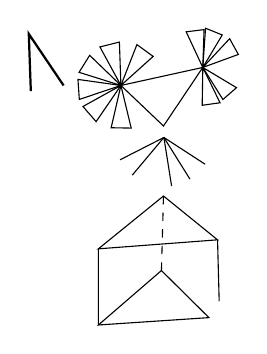
\begin{tikzpicture}[scale=.52]
\draw[thick] (-2.2,2.1)--(-2.25,3.5)--(-1.4,2.24);
\coordinate (u) at (0,2.24);\coordinate (v) at (2,2.68);
\draw (u)--(v)--(1.04,1.25)--(u);
\foreach \a in {42,92,136,172,209,257}{\draw (u)--++(\a:1.06)--++(\a+102:.49)--(u);}
\foreach \a in {47,86,115,-31,-64}{\draw (v)--++(\a:.96)--++(\a-108:.44)--(v);}
\foreach \a in {207,230,279,302,327}{\draw (1.05,.97)--++(\a:1.2);}
\draw (-.55,-1.75)--(1.04,-.46)--(2.36,-1.53)--cycle (-.55,-3.61)--(.99,-2.28)--(2.15,-3.43)--cycle
 (-.55,-3.61)--(-.55,-1.75) (2.36,-1.53)--(2.4,-3.03);
\draw[dashed] (1.04,-.46)--(.99,-2.28);
\end{tikzpicture}}

% L11–14 far right
$\unsure{\zeta_{1i}|\zeta_1\,i|\xi_1}\qquad i\in\{1,\ldots,6\}$

$1\ \underline{1}$

$(2\eta-\zeta)\mathbin{\unsure{\cdot|+}}\unsure{h_j|W_j|\xi_j}=2$

% L14–16 lower middle
\[
 \begin{aligned}
 &\mathfrak S_3\quad\sim\qquad 6^4=2^4\,3^4\quad\text{\textcircled{40}}\\
 &\begin{array}{r}81\\16\\\hline486\\81\phantom0\\\hline1296\end{array}
 \end{aligned}
\]

% L15–18 lower left
\[
 \begin{aligned}
 &\begin{matrix}F\\\downarrow\\E\end{matrix}
 \qquad\coprod_{i\in E}\ \prod_{j\in E-\{i\}}F_j\\
 &\unsure{\zeta'}\qquad \unsure{\zeta}= \eta-\deleted{\unsure{\zeta_j}}\zeta_k
 \end{aligned}
\]

% L18–21 lower centre left
\unsure{ou parties de|ou partitions|on particulier} \deleted{\unsure{telles que|telle que}} de \unsure{Card.|card.} 2 \unsure{jt} qui ne sont pas dans une fibre

% lower left edge
% margin note written sideways
\margin{$2\eta-\zeta\qquad 2\eta-\zeta_i-\zeta_j\qquad 4-2=2\qquad\zeta'_i-\zeta_i$}

% lower right edge
% margin note written sideways
\margin{$\dfrac{27\cdot16\cdot10}{6}=9\cdot16\cdot5=720=6!$}

% lower right L15–20
\figure{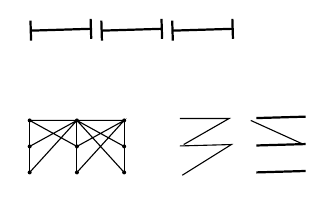
\begin{tikzpicture}[scale=.6]
\foreach \x in {0,1.5,3}{\draw[|-|,thick] (\x,3)--(\x+1.32,3.04);}
\foreach \x in {0,1,2}{\foreach \y in {0,.55,1.1}{\fill (\x,\y) circle (1.2pt);}\draw (\x,0)--(\x,1.1);}
\draw (0,1.1)--(2,1.1) (0,.55)--(1,1.1)--(2,0) (0,0)--(1,1.1)--(2,.55) (0,1.1)--(1,.55)--(2,1.1)--(1,0);
\foreach \y in {0,.57,1.15}{\draw[thick] (4.8,\y)--(5.84,\y+.03);}
\draw (3.18,.56)--(4.27,.59)--(3.23,-.06) (3.18,1.14)--(4.22,1.14)--(3.26,.59) (4.68,1.1)--(5.76,.61);
\end{tikzpicture}}

% bottom centre
\[
 \begin{aligned}&\deleted{\unsure{42}}\\&9\times9=81\\&3\times3\times3=27\\&54\end{aligned}
\]

% foot
\figure{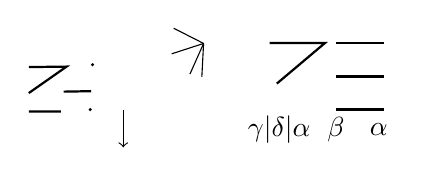
\begin{tikzpicture}[scale=.6]
\draw[thick] (0,.9)--(.8,.91)--(0,.35) (.74,.38)--(1.32,.39) (0,-.04)--(.68,-.04);
\fill (1.35,.95) circle (1pt); \fill (1.3,0) circle (1pt);
\draw[->] (2,0)--(2,-.8);
\foreach \y in {0,.7,1.41}{\draw[thick] (6.5,\y)--(7.52,\y);}
\draw[thick] (5.1,1.41)--(6.27,1.41)--(5.25,.55);
\node at (5.3,-.43) {$\unsure{\gamma|\delta|\alpha}$};\node at (6.5,-.43) {$\beta$};\node at (7.41,-.43) {$\alpha$};
\foreach \a in {153,198,246,267}{\draw (3.7,1.4)--++(\a:.71);}
\end{tikzpicture}}
% archive sheet number: 26
\scanpage{28}

% top hexagon
\diagram{\begin{tikzcd}[ampersand replacement=\&,execute at end picture={\begin{scope}[x=.65cm,y=.65cm]\coordinate (t) at (0,3);
\coordinate (u) at (-2.7,2);
\coordinate (v) at (2.7,2);
\coordinate (w) at (-2.7,0.05);
\coordinate (x) at (2.7,0.05);
\coordinate (b) at (0,-1.12);

\node[above,inner sep=1.2pt] at (t) {$\overbrace{\unsure{\zeta|\xi}_{1}\,\zeta_{2}\,\zeta_{3}}$};
\node[left,inner sep=1.2pt] at (u) {$\zeta_{56}\,\zeta_{64}\,\zeta_{45}$};
\node[right,inner sep=1.2pt] at (v) {$\zeta_{4}\,\zeta_{5}\,\zeta_{6}$};
\node[left,inner sep=1.2pt] at (w) {$\zeta_{1}'\,\zeta_{2}'\,\zeta_{3}'$};
\node[right,inner sep=1.2pt] at (x) {$\zeta_{23}\,\zeta_{31}\,\zeta_{12}$};
\node[below,inner sep=1.2pt] at (b) {$\underbrace{\zeta_{4}'\,\zeta_{5}'\,\zeta_{6}'}$};
\draw (-.87,3)--(-1.48,2.48) (.86,3)--(1.5,2.5) (-3.36,1.57)--(-3.36,.63) (3.38,1.55)--(3.36,.62) (-1.45,-.15)--(-.85,-.73) (1.45,-.15)--(.85,-.74);
\draw[dashed] (t)--(w)--(x)--cycle (u)--(v)--(b)--cycle;\node[right,inner sep=1pt] at (-2.05,2.83) {$r_6$};
\node[right,inner sep=1pt] at (1.33,2.98) {$r_0$};
\node[left,inner sep=1pt] at (-3.49,1.03) {$-r_{456}$};
\node[right,inner sep=1pt] at (3.49,1.03) {$r_{456}=3(r_1+r_2\mathbin{\unsure{+|\circ}}r_3)+2r_4+r_5+r_6$};
\node[left,inner sep=1pt] at (-1.45,-0.69) {$-r_0$};
\node[right,inner sep=1pt] at (1.48,-0.7) {$-r_{123}=-r_6$};\draw[fill=black!24] (2.7,2)--(2.17,2)--(2.43,1.57)--cycle;\foreach \x in {0,.07,.14,.21}{\draw (2.2+\x,1.99)--(2.43,1.59+\x);}\draw[fill=black!17] (2.7,.06)--(2.16,.07)--(2.39,.52)--cycle;\foreach \x in {0,.07,.14,.21}{\draw (2.17+\x,.07)--(2.39+\x/2,.43-\x/2);}\end{scope}}] {} \end{tikzcd}}
\margin{$\begin{gathered}{[r_6,r_0]}\\[-2pt]''\\[-2pt][r_6,r_{456}]\\[-2pt]''\\[-2pt][r_{123},r_{456}]\end{gathered}$}

% middle hexagon
\diagram{\begin{tikzcd}[ampersand replacement=\&,execute at end picture={\begin{scope}[x=.65cm,y=.65cm]\coordinate (t) at (0,3);
\coordinate (u) at (-2.7,2);
\coordinate (v) at (2.7,2);
\coordinate (w) at (-2.7,0.05);
\coordinate (x) at (2.7,0.05);
\coordinate (b) at (0,-1.12);

\node[above,inner sep=1.2pt] at (t) {$\zeta_{1}\,\zeta_{1}'\,\zeta_{23}$};
\node[left,inner sep=1.2pt] at (u) {$\zeta_{34}\,\zeta_{35}\,\zeta_{36}$};
\node[right,inner sep=1.2pt] at (v) {$\zeta_{24}\,\zeta_{25}\,\zeta_{26}$};
\node[left,inner sep=1.2pt] at (w) {$\zeta_{2}\,\zeta_{2}'\,\zeta_{31}$};
\node[right,inner sep=1.2pt] at (x) {$\zeta_{3}\,\zeta_{3}'\,\zeta_{12}$};
\node[below,inner sep=1.2pt] at (b) {$\zeta_{14}\,\zeta_{15}\,\zeta_{16}$};
\draw (-.87,3)--(-1.48,2.48) (.86,3)--(1.5,2.5) (-3.36,1.57)--(-3.36,.63) (3.38,1.55)--(3.36,.62) (-1.45,-.15)--(-.85,-.73) (1.45,-.15)--(.85,-.74);
\draw[dashed] (t)--(w)--(x)--cycle (u)--(v)--(b)--cycle;\node[right,inner sep=1pt] at (-2.05,2.83) {$r_{3,1}=-r_1-r_2$};
\node[right,inner sep=1pt] at (1.33,2.98) {$r_{21}=-r_{12}=-r_1$};
\node[left,inner sep=1pt] at (-3.49,1.03) {$r_{3,2}=-r_2$};
\node[right,inner sep=1pt] at (3.49,1.03) {$r_{2,3}=r_2$};
\node[left,inner sep=1pt] at (-1.45,-0.69) {$r_{1,2}=r_1$};
\node[right,inner sep=1pt] at (1.48,-0.7) {$r_{1,3}=r_1+r_2$};\draw[fill=black!22] (0,3)--(-.35,2.47)--(.18,2.64)--cycle; \foreach \x in {0,.07,.14,.21}{\draw (-.34+\x,2.47+\x)--(.18,2.64+\x/2);}\draw[fill=black!24] (2.7,2)--(2.17,2)--(2.43,1.57)--cycle;\foreach \x in {0,.07,.14,.21}{\draw (2.2+\x,1.99)--(2.43,1.59+\x);}\end{scope}}] {} \end{tikzcd}}
\margin{$[r_1,r_2]$}

% lower hexagon
\diagram{\begin{tikzcd}[ampersand replacement=\&,execute at end picture={\begin{scope}[x=.65cm,y=.65cm]\coordinate (t) at (0,3);
\coordinate (u) at (-2.7,2);
\coordinate (v) at (2.7,2);
\coordinate (w) at (-2.7,0.05);
\coordinate (x) at (2.7,0.05);
\coordinate (b) at (0,-1.12);

\node[above,inner sep=1.2pt] at (t) {$\zeta_{4}\,\zeta_{4}'\,\zeta_{56}$};
\node[left,inner sep=1.2pt] at (u) {$\zeta_{16}\,\zeta_{26}\,\zeta_{36}$};
\node[right,inner sep=1.2pt] at (v) {$\zeta_{15}\,\zeta_{25}\,\zeta_{35}$};
\node[left,inner sep=1.2pt] at (w) {$\zeta_{5}\,\zeta_{5}'\,\zeta_{64}$};
\node[right,inner sep=1.2pt] at (x) {$\zeta_{6}\,\zeta_{6}'\,\zeta_{45}$};
\node[below,inner sep=1.2pt] at (b) {$\zeta_{14}\,\zeta_{24}\,\zeta_{34}$};
\draw (-.87,3)--(-1.48,2.48) (.86,3)--(1.5,2.5) (-3.36,1.57)--(-3.36,.63) (3.38,1.55)--(3.36,.62) (-1.45,-.15)--(-.85,-.73) (1.45,-.15)--(.85,-.74);
\draw[dashed] (t)--(w)--(x)--cycle (u)--(v)--(b)--cycle;\node[right,inner sep=1pt] at (-2.05,2.83) {$r_{6,4}=-r_4-r_5$};
\node[right,inner sep=1pt] at (1.33,2.98) {$r_{5,4}=-r_{45}=-r_4$};
\node[left,inner sep=1pt] at (-3.49,1.03) {$r_{6,5}=-r_5$};
\node[right,inner sep=1pt] at (3.49,1.03) {$r_{5,6}=r_5$};
\node[left,inner sep=1pt] at (-1.45,-0.69) {$r_{4,5}=r_4$};
\node[right,inner sep=1pt] at (1.48,-0.7) {$r_{4,6}=r_4+r_5$};\draw[fill=black!22] (0,3)--(-.35,2.47)--(.18,2.64)--cycle; \foreach \x in {0,.07,.14,.21}{\draw (-.34+\x,2.47+\x)--(.18,2.64+\x/2);}\draw[fill=black!24] (2.7,2)--(2.17,2)--(2.43,1.57)--cycle;\foreach \x in {0,.07,.14,.21}{\draw (2.2+\x,1.99)--(2.43,1.59+\x);}\end{scope}}] {} \end{tikzcd}}
\margin{$[r_4,r_5]$}

% line below third hexagon
$\overline{r_1\,r_2}\quad\overline{r_4,r_5}\quad r_0,r_6$ \unsure{engendre|engendrent} un sous groupe d'indice 3 dans $E$

\deleted{$[r_1,r_2]\quad [$}

% foot left
\diagram{\begin{tikzcd}[ampersand replacement=\&,column sep=small,row sep=small]
 r_1\arrow[r,dash]\&r_2\arrow[r,dash]\&r_3\arrow[r,dash]\arrow[d,dash]\&r_4\arrow[r,dash]\&r_5\\
 \&\&\unsure{\delta_6|r_6}\&\&
\end{tikzcd}}

% foot centre
\diagram{\begin{tikzcd}[ampersand replacement=\&,execute at end picture={\begin{scope}[x=.7cm,y=.7cm]\coordinate (o000) at (0,4);
\coordinate (o001) at (0.68,4);
\coordinate (o002) at (1.36,4);
\coordinate (o010) at (0,3.35);
\coordinate (o011) at (0.68,3.35);
\coordinate (o012) at (1.36,3.35);
\coordinate (o020) at (0,2.7);
\coordinate (o021) at (0.68,2.7);
\coordinate (o022) at (1.36,2.7);
\coordinate (o100) at (4,4);
\coordinate (o101) at (4.68,4);
\coordinate (o102) at (5.36,4);
\coordinate (o110) at (4,3.35);
\coordinate (o111) at (4.68,3.35);
\coordinate (o112) at (5.36,3.35);
\coordinate (o120) at (4,2.7);
\coordinate (o121) at (4.68,2.7);
\coordinate (o122) at (5.36,2.7);
\coordinate (o200) at (2,1.7);
\coordinate (o201) at (2.68,1.7);
\coordinate (o202) at (3.3600000000000003,1.7);
\coordinate (o210) at (2,1.0499999999999998);
\coordinate (o211) at (2.68,1.0499999999999998);
\coordinate (o212) at (3.3600000000000003,1.0499999999999998);
\coordinate (o220) at (2,0.3999999999999999);
\coordinate (o221) at (2.68,0.3999999999999999);
\coordinate (o222) at (3.3600000000000003,0.3999999999999999);

\node[anchor=center,inner sep=1.2pt] at (o000) {$\zeta_{1}$};
\node[anchor=center,inner sep=1.2pt] at (o001) {$\zeta_{2}$};
\node[anchor=center,inner sep=1.2pt] at (o002) {$\zeta_{3}$};
\node[anchor=center,inner sep=1.2pt] at (o010) {$\zeta_{1}'$};
\node[anchor=center,inner sep=1.2pt] at (o011) {$\zeta_{2}'$};
\node[anchor=center,inner sep=1.2pt] at (o012) {$\zeta_{3}'$};
\node[anchor=center,inner sep=1.2pt] at (o020) {$\zeta_{23}$};
\node[anchor=center,inner sep=1.2pt] at (o021) {$\zeta_{31}$};
\node[anchor=center,inner sep=1.2pt] at (o022) {$\zeta_{12}$};
\node[anchor=center,inner sep=1.2pt] at (o100) {$\zeta_{4}'$};
\node[anchor=center,inner sep=1.2pt] at (o101) {$\zeta_{5}'$};
\node[anchor=center,inner sep=1.2pt] at (o102) {$\zeta_{6}'$};
\node[anchor=center,inner sep=1.2pt] at (o110) {$\zeta_{4}$};
\node[anchor=center,inner sep=1.2pt] at (o111) {$\zeta_{5}$};
\node[anchor=center,inner sep=1.2pt] at (o112) {$\zeta_{6}$};
\node[anchor=center,inner sep=1.2pt] at (o120) {$\zeta_{56}$};
\node[anchor=center,inner sep=1.2pt] at (o121) {$\zeta_{64}$};
\node[anchor=center,inner sep=1.2pt] at (o122) {$\zeta_{45}$};
\node[anchor=center,inner sep=1.2pt] at (o200) {$\zeta_{14}$};
\node[anchor=center,inner sep=1.2pt] at (o201) {$\zeta_{15}$};
\node[anchor=center,inner sep=1.2pt] at (o202) {$\zeta_{16}$};
\node[anchor=center,inner sep=1.2pt] at (o210) {$\zeta_{24}$};
\node[anchor=center,inner sep=1.2pt] at (o211) {$\zeta_{25}$};
\node[anchor=center,inner sep=1.2pt] at (o212) {$\zeta_{26}$};
\node[anchor=center,inner sep=1.2pt] at (o220) {$\zeta_{34}$};
\node[anchor=center,inner sep=1.2pt] at (o221) {$\zeta_{35}$};
\node[anchor=center,inner sep=1.2pt] at (o222) {$\zeta_{36}$};
\foreach \y in {4,3.35,2.7}{\draw[thick] (1.86,\y)--(2.96,\y);}
\draw (0,2.48)..controls (.02,2.18) and (.67,1.75).. (1.62,1.7)
 (.67,2.43)..controls (.58,1.43) and (.97,1.19)..(1.66,1.06)
 (1.38,2.47)..controls (1.05,1.4) and (1.16,.59)..(1.69,.4);
\foreach \x in {0,.68,1.36}{\draw (4+\x,2.45)..controls (3.87+\x,2.1) and (2.43+\x,2.28)..(2.06+\x,1.99);}\end{scope}}] {} \end{tikzcd}}
% archive sheet number: 27
\scanpage{29}

% L1–9 top
\deleted{\uline{Prop.} Les \deleted{\unsure{3 bases|bitriades}} \inserted{parties 3-libres} ordonnées sont conjuguées. Si}

\deleted{$J$ est une telle partie, $\exists$ exactement deux bases qui la contiennent, soit $I$ et $I'$, et $\underbrace{(I-J)}_{K}\cup\underbrace{(I'-J)}_{K'}$ est de cardinal 6, et formé de l'ens des \unsure{$\delta$ de $S$|$\delta\in\Delta-J$} qui ne sont liés à aucun él. de $K$. De plus, $\exists!$ bibase $I\cup I'$ contenant $K\cup K'$, et $K,K'$ sont respect\textsuperscript{t} les int. de $I,I'$ avec $K\cup K'$, et \deleted{\unsure{ils sont conjugués}} \inserted{$\exists$ donc \unsure{$K\cup K'$ est stable}}, \deleted{\unsure{correspondance} par \unsure{$t$|$\sigma$} (l'unique autom $\ne\mathrm{id}$ qui \unsure{ne bouge pas|respecte|fixe} la bibase \ldots)} et si}

% L10–11
\[
 \begin{aligned}
 J&=\deleted{\{\lambda_{45},\lambda_{56},\lambda_{61}\}}\\
 K\cup K'&:\ \deleted{\{\underbrace{\unsure{\zeta|\xi}_1,\zeta_2,\zeta_3}_{K},
 \underbrace{\zeta'_1,\zeta'_2,\zeta'_3}_{K'}\}}
 \end{aligned}
\]

% L12–13
\[
 \begin{aligned}
 &\deleted{6!=720=2^4\,3^2\,5}\qquad72\ \text{bases}\quad/\ \underline{36\ \text{bibases}}\\
 &\deleted{6^4=2^4\,3^4=1296}\qquad40\ \text{trihexagones}
 \end{aligned}
 \qquad\begin{array}{r}36\\36\\\hline216\\108\phantom0\\\hline1296\end{array}
\]

% L14–17 left
\[
 \begin{array}{lr}\text{sommets}&27\\\text{bibases}&36\\
 \text{trihexagones}&40\\\text{triangles}&45\end{array}
\]

% middle
\figure{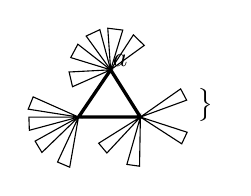
\begin{tikzpicture}[scale=.6]
\coordinate (a) at (0,1);\coordinate (b) at (-.68,0);\coordinate (c) at (.63,0);
\draw[very thick] (a)--(b)--(c)--cycle;
\foreach \ang in {36,73,105,142,183}{\draw (a)--++(\ang:.88)--++(\ang+100:.32)--cycle;}
\foreach \ang in {156,180,209,245}{\draw (b)--++(\ang:1.05)--++(\ang+92:.28)--cycle;}
\foreach \ang in {35,-18,-91,-133}{\draw (c)--++(\ang:1.04)--++(\ang-97:.27)--cycle;}
\node at (.2,1.19) {$\unsure{a}$};\node at (2,.25) {$\big\}$};
\end{tikzpicture}}

% L14–19 middle right
\[
 \begin{aligned}
 &\unsure{\mathfrak S|\mathfrak G}_4\\
 &\deleted{\unsure{4|2}}\mathfrak S_3/\mathfrak S_4/\mathbb F_2^{\unsure{3}}\\
 &72\cdot24\\&2^{\unsure{7}}\cdot9
 \end{aligned}
\]

% L18–21 lower left
$\mathfrak S_4\ \mathbb F_2^4\quad\mathrm{ord.}\quad24\cdot16$

\unsure{qui fixe|quadriques} deux droites $3$ sur $\mathbb F_2$

$8\cdot\mathrm{G\unsure{L|l}}(3,\mathbb F_2)$

$\deleted{\unsure{P(i)}}\quad\deleted{\unsure{2}}\quad 8-2/2=3$

% L18–21 lower centre
$A(i)$ ens à 4 él. \quad $i\in T$

$P(i)$ torseur sous $\unsure{V(i)|k(i)}=\mathbb F_2^{A(i)}\quad\left.\vphantom{\mathbb F_2^{A(i)}}\right\}\text{ à 16 él.)}$

$\forall i$, bijection entre $P(i)$ et $\displaystyle\coprod_{j\in T-\{i\}}\ \unsure{\alpha}\in A(j)$

% L22–26 left
\[
 \begin{aligned}
 &P(i)/\deleted{\unsure{W|V}}V'(i)\simeq T-\{i\}\\
 &(1+q)(1+q^{\unsure{2|-1}})\,q^{3}(q-1)^2\qquad q=2\\
 &2^3\cdot3\cdot5\mathbin{\unsure{=|.}}\underline{120}\ !!!\quad\deleted{P(i)}\\
 &20
 \end{aligned}
\]

% L22–26 centre
\diagram{\begin{tikzcd}[ampersand replacement=\&,column sep=small,row sep=small]
 {}\arrow[r,dash]\& k\arrow[r,phantom,"\scriptstyle\subset" description]\&V'(i)\arrow[r,phantom,"\scriptstyle\subset" description]\&V(i)\arrow[r,dash]\&0\\
 {}\arrow[r,dash]\& {}\arrow[r,dash]\& {}\arrow[r,dash]\&{}\\
 1\&2\&1
\end{tikzcd}}

% L24–27 centre
\diagram{\begin{tikzcd}[ampersand replacement=\&,execute at end picture={\begin{scope}[x=.72cm,y=.72cm]\coordinate (a) at (1.25,0);
\coordinate (b) at (1,1.3);
\coordinate (c) at (0,0);
\draw[->] (a)--(b);
\draw (a)--(c);
\draw[dashed] (b)--(c);
\fill (a) circle (1.15pt);\node[right,inner sep=1.2pt] at (a) {$a$};
\fill (b) circle (1.15pt);\node[above,inner sep=1.2pt] at (b) {$b$};
\fill (c) circle (1.15pt);\node[left,inner sep=1.2pt] at (c) {$c$};
\end{scope}}] {} \end{tikzcd}}

% L24–29 centre right
$V'(i)\quad \deleted{\unsure{V^+(i)|V'(i)}}\quad\unsure{\Gamma_i|P_i}$

$\begin{matrix}k\subset V'\\ \downarrow\\ \mathrm{Aut}(E)\end{matrix}$

% L27–30 lower right
\[
 \begin{matrix}&A_1&\\A_3&&A_2\\\multicolumn{3}{c}{\underbrace{\hspace{3em}}_{\text{3 ens. à 4 él.}}}\end{matrix}
\]

% L29–31 lower left
$V$ vectoriel de dim 3 sur $\mathbb F_2$ \unsure{et}

$\underset{\scriptscriptstyle k}{V}\simeq\underset{\scriptscriptstyle k}{K(A_i)'}$ pour tt $i$\qquad $A_3\times$

% foot right
$V\supset k$ vectoriel de dim 3 sur $\mathbb F_2$
% archive sheet number: 28
\scanpage{30}

% L1–2 upper left
\[
 \begin{matrix}\unsure{\zeta|\xi}_1&\zeta_2&\zeta_3&\zeta_{32}\\
 \zeta'_1&\zeta'_2&\zeta'_3&\end{matrix}
\]

% L1 upper centre
\figure{\begin{tikzpicture}\draw[|-|] (0,0)--(1.65,0);\draw[|-|] (1.7,0)--(3.4,0);\end{tikzpicture}}

% L1 upper right
\[
 \frac{72\cdot6!=72\cdot720}{72\cdot6}=120
\]

% L3–4 left
\diagram{\begin{tikzcd}[ampersand replacement=\&,column sep=small]
 \zeta_1\zeta_2\zeta_3 \& \zeta_4\zeta_5\zeta_6\arrow[r,dash]\& \underline{\zeta_{12}\zeta_{23}\zeta_{34}}\\
 \zeta'_1\zeta'_2\zeta'_3 \& \zeta'_4\deleted{\unsure{*}}\zeta'_5\zeta'_6\arrow[ur,dash]\&\zeta_{45}\zeta_{56}\zeta_{6\unsure{1|4}}
\end{tikzcd}}

% L2–8 upper right
\diagram{\begin{tikzcd}[ampersand replacement=\&,row sep=1ex,column sep=1em,execute at end picture={\draw ([xshift=2pt]current bounding box.north east)--([xshift=-3pt,yshift=-3pt]current bounding box.north west)--([xshift=-3pt,yshift=3pt]current bounding box.south west)--(current bounding box.south east);} ]
 \text{trièdres}\arrow[r,leftrightarrow]\&\text{hexagones}\\
 \text{hex. trièdres}\arrow[r,leftrightarrow]\arrow[d,leftrightarrow]\&\text{bitriangles}\arrow[d,leftrightarrow]\\
 \text{plan } A_2\arrow[r,leftrightarrow]\&\text{bloc de trièdres}\\
 \text{trihexatrièdres}\arrow[r,leftrightarrow]\arrow[d,leftrightarrow]\& \deleted{\unsure{\text{trièdres}}}\,\text{\unsure{triplets|triples de} bitriangles}\arrow[d,leftrightarrow]\\
 \text{décomposition}\arrow[r,dash]\arrow[d,leftrightarrow]\&\text{\unsure{triplet|triple} \unsure{tribloc|bloc} de trièdres}\\
 \deleted{\unsure{\text{triple }A_2|A_2\,\ldots\,A_2}}\ \text{triplan } A_2 \&
\end{tikzcd}}

% centre left
\diagram{\begin{tikzcd}[ampersand replacement=\&,row sep=2ex,column sep=1em]
 \&\underline{\zeta_{12}\zeta_{23}\zeta_{34}}\arrow[dl,dash,"-r_6"']\arrow[dr,dash,"r_{456}"]\&\\
 \zeta'_4\zeta'_5\zeta'_6\arrow[d,dash,"{-r_{\deleted{\unsure{6}}0}} "']\&\&\zeta_4\zeta_5\zeta_6\arrow[d,dash,"r_0"]\\
 \zeta'_1\zeta'_2\zeta'_3\arrow[dr,dash,"-r_{456}"']\&\&\zeta_1\overline{\zeta_2}\zeta_3\arrow[dl,dash,"r_6"]\\
 \&\underline{\zeta_{45}\zeta_{56}\zeta_{61}}\&
\end{tikzcd}}

% centre right
\[
 \zeta_{ij}\quad\begin{matrix}1\le i\le3\\4\le j\le6\end{matrix}
 \qquad
 \begin{matrix}\zeta_{14}&\zeta_{15}&\zeta_{16}\\\zeta_{24}&\zeta_{25}&\zeta_{\underline{26}}\\\zeta_{34}&\zeta_{35}&\zeta_{36}\end{matrix}
\]

% centre below hexagon
\figure{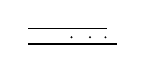
\begin{tikzpicture}[scale=.5]\draw (0,.4)--(2,.4) (0,0)--(2.25,0);\foreach \x in {1.1,1.57,1.96}{\fill (\x,.17) circle (.8pt);}\end{tikzpicture}}

% L10–12
NB de 3 bases (\unsure{ou couples|un couple} de racines : $60^\circ$)

% L11–13
\[
 36\cdot\underbrace{\binom63\deleted{\unsure{2/2|4/24}}}_{\frac{6\cdot5\cdot4}{3!\,\unsure{2^2|2!}}=20}=720
 \qquad\begin{aligned}&\text{nb de paires de}\\&\text{racines faisant }60^\circ\end{aligned}
\]

% L14
plan $A_2$ : $\dfrac{720}{6}=120$ \(\mathbin{/\mkern-4mu/}\)

% lower right
\[
 \begin{matrix}
 \zeta_{14}&\zeta_{25}&\zeta_{36}\\
 \zeta_{26}&\zeta_{34}&\zeta_{15}\\
 \zeta_{35}&\zeta_{16}&\zeta_{24}
 \end{matrix}
\]

% lower left
\diagram{\begin{tikzcd}[ampersand replacement=\&,row sep=1ex,column sep=small]
 \deleted{\text{plan }A_2}\&\\
 \text{sous syst. }A_2\arrow[d,leftrightarrow]\&\\
 \text{\unsure{3bloc|3 blocs} de \unsure{3trièdres|bitriades}}\arrow[d,leftrightarrow]\&
 \unsure{\mathfrak S|\mathfrak G}_2\cdot(\mathfrak S_3\times\mathfrak S_3)\\
 \text{bitriangle}\arrow[d,leftrightarrow]\arrow[ur,phantom,"\smash{\raisebox{.7ex}{$\left.\rule{0pt}{4.3ex}\right\}$}}" description]\& \mathfrak S_3\cdot(\mathfrak S_3\times\mathfrak S_3\times\mathfrak S_3)\\
 \text{hexagone de trièdres.}\&
\end{tikzcd}}

% foot right
\[
 \begin{matrix}
 \bullet\\[-2pt]\triangle\\[-2pt]\cdot\ \cdot\ \cdot\ \cdot\ \cdot\ \cdot\\[-2pt]
 \deleted{\unsure{\boxplus}}\ \text{\unsure{tribloc|triple}}
 \end{matrix}
 \quad
 \left\{\begin{array}{lr}
 \text{sommets}&27\\\text{triangles}&45\\\text{bibase}&36\\\text{trois-neufs}&40
 \end{array}\right.
\]
% archive sheet number: 29
\scanpage{31}

% L1–3 across top
\diagram{\begin{tikzcd}[ampersand replacement=\&,row sep=3.4ex,column sep=.2em,font=\scriptsize,
 execute at end picture={\draw (\tikzcdmatrixname-1-1.west) .. controls ++(-.75,-.1) and ++(-.6,.5) .. (\tikzcdmatrixname-2-1.west);
 \draw (\tikzcdmatrixname-1-1.south) .. controls ++(-.8,-.26) and ++(-.65,.8) .. (\tikzcdmatrixname-3-1.west);
 \draw (\tikzcdmatrixname-2-2.south) .. controls ++(.6,-.3) and ++(-.25,1.1) .. (\tikzcdmatrixname-2-2.east);}]
\big[\;(\unsure{\zeta|\xi}_{1}\zeta_{2}\zeta_{3})(\deleted{\unsure{1}}\zeta'_{4}\zeta'_{5}\zeta'_{6})\arrow[d,dash,"{\zeta_3}"]\arrow[dr,dash] \& (\zeta_{4}\zeta_{5}\zeta_{6})(\zeta'_{1}\zeta'_{2}\zeta'_{3})\arrow[dl,dash,"{\zeta_1}"]\arrow[d,dash,"{\zeta_2}"]\arrow[dr,dash,"{\zeta_3}"]\arrow[ddl,dash,"{\zeta_4}"]\arrow[dd,dash,"{\zeta_5}"]\arrow[ddr,dash,"{\zeta_6}"] \& (\zeta_{23}\zeta_{31}\zeta_{12})(\zeta_{56}\zeta_{\unsure{64|61}}\zeta_{45}) \\
\big[\;(\zeta_{1}\zeta'_{1}\zeta_{23})(\zeta_{14}\zeta_{15}\zeta_{16}) \& (\zeta_{24}\zeta_{25}\zeta_{26})(\zeta_{2}\zeta'_{2}\zeta_{31}) \& (\zeta_{3}\zeta'_{3}\zeta_{12})(\zeta_{34}\zeta_{35}\zeta_{36}) \\
\big[\;(\zeta_{4}\zeta'_{4}\zeta_{56})(\zeta_{14}\zeta_{24}\zeta_{34}) \& (\zeta_{5}\zeta'_{5}\zeta_{64})(\zeta_{15}\zeta_{25}\zeta_{35}) \& (\zeta_{6}\zeta'_{6}\zeta_{45})(\zeta_{16}\zeta_{26}\zeta_{36})
\end{tikzcd}}

% left between L2 and L3
$\deleted{\unsure{\zeta_{12}}}$
% archive sheet number: 30
\scanpage{33}

% L1–2
$V$ groupe comm. (écrit additivement)

$I$ ens de cardinal 3

% L3
\[
 \Gamma=\mathrm{Ker}\,(V^I\to V)
\]

% L4
$\omega$ ens des \inserted{\unsure{2|?}} ordres circulaires sur $I$ (c'est un $(\pm1)$-\unsure{tors|tors.})

% L5
\[
 V^\omega=V\mathbin{\wedge}_{\{\pm1\}}\omega
 \qquad(\pm1\text{ opérant sur }V\text{ par chg}\textsuperscript{t}\text{ de signe})
\]

% L6–9
Pour $i\in I$, \unsure{---}
\[
 V^\omega\xrightarrow{\varphi_i}\Gamma\quad\text{par}\quad\deleted{(x,\rho)}
 \left\{\begin{aligned}
 &\varphi_i(x\wedge\rho)_{\deleted{\unsure{\rho}}i}=0\\
 &\varphi_i(x\wedge\rho)_{\rho i}=x\\
 &\varphi_i(x\wedge\rho)_{\rho^2 i}=-x
 \end{aligned}\right.
\]

% L6–10 right
\margin{\uline{NB} \(\deleted{\unsure{\varphi_i(x)+\varphi_{\rho i}(x)+\varphi_{\rho^2 i}(x)=0}}\)
\(\displaystyle\sum_{i\in I}\varphi_i(x)=0\quad\forall x\in V^\omega\)}

% L10
On cherche à obtenir les systèmes

% L11–13
\deleted{\unsure{et|$\psi$}}
\diagram{\begin{tikzcd}[ampersand replacement=\&]
 V^\omega\arrow[r,dash,"\varphi_i"]\arrow[dr,"\psi_i"']\&\Gamma\\
 \&\widetilde\Gamma^{\unsure{''|*}}\arrow[u,"{\unsure{u|k}}"']
\end{tikzcd}}

% L10–14 right
\margin{\deleted{\uline{NB}} En fait, on a suite exacte
\(\begin{gathered}0-V^\omega\xrightarrow[\mathrm{diag}]{}(V^\omega)^I\to\Gamma-0\\
\text{i.e.}\\
0-V^\omega-(V^\omega)^I\to V^I\to V\to0\end{gathered}\)}

% L14–17
avec

\deleted{\unsure{i}} a) $\widetilde\Gamma\xrightarrow{u}\Gamma$ est un hom de groupes à noyau central $Z$

b) $\psi_i$ un hom $V^\omega\mathbin{\unsure{-|\to}}\widetilde\Gamma$ qui relève $\varphi_i$ :

% L18
\[
 u\psi_i=\varphi_i
\]

% L19–20
\uline{NB} $u$ doit être épi, donc $\widetilde\Gamma$ est une \uline{extension} de $\Gamma$ par $Z$ (écrit addit\textsuperscript{\unsure{mt}})

% L21
Soit $\rho\in\omega$, $i_0\in I$, d'où $i_1=\rho i_0,\ i_2=\rho^2i_0=\rho i_1$. On aura

% L22
\[
 \varphi_{i_0}(\deleted{\unsure{X}}x\wedge\rho)+\varphi_{i_1}(x\wedge\rho)+\varphi_{i_2}(x\wedge\rho)=0
\]

% L23
d'où
\[
 \psi_{i_0}(x\wedge\rho)\,\psi_{i_1}(x\wedge\rho)\,\psi_{i_2}(x\wedge\rho)
 =z(x,\rho,i_0)\in Z.
\]
% archive sheet number: 32
\scanpage{34}

% L1–3
On a, comme $Z$ est central
\[
 \begin{aligned}
 z(x,\rho,i_0)&=z(x,\rho,i_1)=z(x,\rho,i_2)\\
 \text{Soit}\qquad&=z(x,\rho)=z_\rho(x)
 \end{aligned}
\]

% L4–6
D'ailleurs on aura
\[
 \begin{aligned}
 &\psi_{i_2}(\deleted{\unsure{2}}x\wedge\rho)^{-1}\,\psi_{i_1}(x\wedge\rho)^{-1}\,
 \psi_{i_0}(x\wedge\rho)^{-1}=-z(x,\rho)\\
 \text{i.e.}\quad&\psi_{i_2}((-x)\wedge\rho)\,\psi_{i_1}((-x)\wedge\rho)\,
 \psi_{i_0}((\unsure{+|-}x)\wedge\rho)=-z(x,\rho)
 \end{aligned}
\]

% L7–8
i.e. \deleted{\unsure{toujours|compte tenu}} comme $(-x)\wedge\rho=x\wedge\bar\rho^{\deleted{\unsure{2}}}$
$(\bar\rho=\rho^2=\rho^{-1})$
\[
 \psi_{i_2}(x\wedge\bar\rho)\,\psi_{i_1}(x\wedge\bar\rho)\,\psi_{i_0}(x\wedge\bar\rho)
 =-z(x,\rho)
\]

% L9–10
i.e. on a
\[
 z(x,\bar\rho)=-z(x,\rho)\qquad\text{i.e.}\quad z_{\bar\rho}=-z_\rho
\]

% L11–14
i.e on a deux applications
\[
 z_\rho:V^{\deleted{\unsure{\omega}}}\longrightarrow Z\qquad \rho\in\omega
\]
différant par le signe, (i.e. un élément de $(Z^V)\wedge_{\pm1}\omega$). \deleted{On aura}

% L15–17
\uline{Prop.} On aura
\[
 \left\{\begin{aligned}
 &\deleted{z_\rho(0)=0\quad\text{et}}\quad\text{si}\quad j=\rho i\\
 &\varphi_i(x)\varphi_j(y)\varphi_i(x)^{-1}\varphi_j(y)^{-1}
 =z_\rho(x)+z_\rho(y)-z_\rho(x+y)
 \end{aligned}\right.
\]

% L18
L'application $\lambda=z_\rho\unsure{=:|:}V\mathbin{\unsure{-|\to}}Z$ satisfait

% L19–21
\[
 \left\{\begin{aligned}
 &\deleted{z_\rho}\lambda(0)=0\\
 &\begin{aligned}
 &\deleted{z_\rho}\lambda(x)+\deleted{z_\rho}\lambda(y+\unsure{u|u'})
 +\deleted{z_\rho}\lambda(y+\unsure{v|v'})+\deleted{z_\rho}\lambda(x+\unsure{u'|u}+v)\\
 &\quad=\deleted{z_\rho}\lambda(y)+\deleted{z_\rho}\lambda(x+u)
 +\deleted{z_\rho}\lambda(x+v)+\deleted{z_\rho}\lambda(y+\unsure{u'|u}+v)
 \end{aligned}
 \end{aligned}\right. \tag*{$(\unsure{*|\star})$}
\]
% archive sheet number: 33
\scanpage{35}

% printed form left column, head
% printed form
N\textsuperscript{o}

UNIVERSITÉ DES SCIENCES\\
ET TECHNIQUES\\
DU LANGUEDOC

% printed form left column, (1)
(1) -- Le candidat doit indiquer la nature de l'examen auquel il se présente.

% printed form left column, (2)
(2) -- Le candidat inscrit ses nom, prénom, lieu et date de naissance en tête de la copie et signe lisiblement son nom à la fin de la composition.

% printed form main column, head
ACADEMIE DE MONTPELLIER

% printed form main column, L2–3
\textit{Examen de} \textsuperscript{(1)} \dotfill\\
\mbox{}\dotfill

% printed form main column, L4–7
\textit{Nom et Prénoms du Candidat} \textsuperscript{(2)} \dotfill

\textit{né à} \dotfill\quad \textit{département de} \dotfill

\textit{le} \dotfill\quad 19

\textit{Montpellier, le} \dotfill\quad 19

% printed form main column, last line
COMPOSITION EN \dotfill
% archive sheet number: 34
\scanpage{36}

% L1–3
ou encore (pour la 2\textsuperscript{\unsure{ième|ème}} relation)
\[
 \begin{aligned}
 &\lambda(x+u+v)-\lambda(x+u)-\lambda(x+v)+\lambda(x)\\
 &\qquad=\lambda(y+u+v)-\lambda(y+u)-\lambda(y+v)+\lambda(y
 \end{aligned}
\]

% L4–6
\[
 (\Delta_{uv}\lambda)(x)=\mathrm{c}^{\mathrm{te}}\quad(\text{pour }u,v\text{ fixés})
\]
i.e. \deleted{\unsure{Pour poser}}, posant
\[
 \lambda(u+v)-\lambda(u)-\lambda(v)=\mu(u,v)
\]

% L7–8
On doit avoir
\[
 \boxed{\lambda(x+u+v)-\lambda(\unsure{x+u})-\lambda(\unsure{x+v})+\lambda(x)=\mu(u,v)}
\]

% L9–10
i.e. $\mu$ est \uline{bi-additive}.

\deleted{$\lambda(x+u+v)=\lambda(\unsure{u})+\lambda(v)$}

% L11–14
Pour $\mu$ \inserted{(\unsure{Z|2}-bilinéaire symétrique)} \unsure{fixée|fixé}, les $\lambda$ satisfaisant la relation précédente \inserted{et telles que $\lambda(0)=0$} forment un torseur sous l'ens des $f$ telles que

% L14–16
\[
 \left\{\begin{aligned}
 &f(0)=0\\
 &f(\deleted{\unsure{u}}x+u+v)-f(x+u)-f(x+v)\deleted{\unsure{+f(x)}}=0
 \end{aligned}\right.
\]

% L16–19
\inserted{telles que}

\deleted{i.e. $f(x)+f(y)$ ne dépend que de $x+y$, i.e. \unsure{$\exists g:V\to Z$} telle que \unsure{$f(x)+f(y)=f(x+y)$|$f(x+y)+f(0)=f(x$}}

\deleted{\unsure{pour le}} i.e. $f$ est un \deleted{\unsure{f|affine}} \uline{hom}.

% L20–26
\deleted{\unsure{Dans le cas que}} Lorsque $V$ est un module libre sur un $\mathbb Z/n\mathbb Z$, alors \uline{tte} \uline{\unsure{appl.|produit}} bil. sym. de $V$ dans un $Z$ est associée à une forme quadratique (définie mod application \uline{additive}) \unsure{ssi|sss} les $\mu(e_i,e_i)\in2Z$ ($(e_i)$ est une base de $V$ sur $\mathbb Z/n\mathbb Z$) \unsure{en|ou}
% archive sheet number: 35
\scanpage{37}

% printed letterhead upper left
% letterhead
UNIVERSITE DES SCIENCES ET TECHNIQUES\\
DU LANGUEDOC\\
LABORATOIRE DE SPECTROMÉTRIE I. R.\\
Place Eugène Bataillon\\
34060 MONTPELLIER CEDEX\\
Tél. : 63.91.44\quad (Poste 473)\\
R. BRUNEL, Maître de Conférences\\

% upper right date
Montpellier, le\qquad 14 Juin 1977\\

% upper right address
Monsieur \handwritten{le Professeur GROTHENDIEK}\\

% salutation
Cher Collègue,\\

% body L1–4
La délibération d'admissibilité du jury du DEUG A 1ère Année Série I est fixée au lundi 27 Juin 1977 à 14 h 30, salle 1TC1P . Les délibérations des deux autres séries auront lieu en même temps dans les salles voisines .

% body L5–6
En votre qualité de membre de ce jury , j'ai l'honneur de vous inviter à participer à cette délibération .

% body L7–12
Pour accélérer le déroulement des débats il serait souhaitable que les responsables pédagogiques préparent à l'avance les notes qui doivent figurer sur les procès verbaux compte tenu : des notes des examens partiels, des coefficients de chaque épreuve, des absences motivées aux partiels, des dispenses régulières ...etc... en application des textes officiels relatifs aux modalités du contrôle des connaissances .

% closing L13–14
Je vous prie d'agréer, mon cher collègue, l'expression de mes\\
sentiments amicaux .\\

% signature
Le Président du Jury\\
R.BRUNEL.\qquad\handwritten{\unsure{Brunel}}\\

% postscript L1–2
P.S. La salle 1TC1P est située derrière la salle de cours n\textsuperscript{o} \unsure{8|\S|B} entre le Bâtiment Physique \deleted{\unsure{E|R}}Recherche et le Bâtiment Physique Extension
% archive sheet number: 36
